\documentclass{TIJMUjiaoanLL}
\pagestyle{empty}

\begin{document}

\kecheng{分子生物计算}
\neirong{Perl语言入门 \ / 第2章}
\jiaoshi{伊现富}
\zhicheng{讲师}
\riqi{2018年11月14日15:30-17:10}
\duixiang{生物医学工程与技术学院2016级生信班(本)}
\renshu{28}
\fangshi{理论讲授}
\xueshi{2}
\jiaocai{Perl语言在生物信息学中的应用——基础篇}

\firstHeader
\maketitle
\thispagestyle{empty}

\mudi{
\begin{itemize}
  \item 掌握:Perl的基本知识和语法;三种基本变量;常见操作符。
  \item 熟悉:Perl的基本函数;Perl脚本检修。
  \item 了解:Perl的判断语句和循环语句。
  \item 自学:perltidy的使用;Perl调试器。
\end{itemize}
}

\fenpei{
\begin{itemize}
  \item (5')引言与导入:简单介绍计算机、计算机程序和编程语言的概念。
  \item (10')Perl简介:介绍Perl的基本知识——特性、应用领域、版本、安装与学习等,通过实例介绍Perl的基本语法。
  \item (15')变量:介绍Perl中的三种基本变量——标量、数组和散列,通过实例讲解它们的使用,介绍常见的内置变量。
  \item (15')操作符:介绍数字、字符串、逻辑运算、文件测试和匹配操作符。
  \item (10')基本函数:通过实例讲解print、chomp、join、split、open、close和my等基本函数。
  \item (10')判断语句:通过实例讲解if、unless、和given-when等条件语句。
  \item (15')循环语句:通过实例讲解foreach、for、while和until等循环语句。
  \item (5')脚本检修:介绍检修Perl脚本和格式化代码的基本方法。
  \item (5')总结与答疑:总结授课内容中的知识点与技能,解答学生疑问。
\end{itemize}
}

\zhongdian{
\begin{itemize}
  \item 重点:Perl的基本语法;Perl的三种基本变量。
  \item 难点:Perl的三种基本变量。
  \item 解决策略:通过实例演示帮助学生理解、记忆。
\end{itemize}
}

\waiyu{
\vspace*{-10pt}
\begin{multicols}{3}
脚本(script)

变量(variable)

标量(scalar)

数组(array)

散列(hash)
\end{multicols}
\vspace*{-10pt}
}

\fuzhu{
\begin{itemize}
  \item 多媒体:Perl的标识,基本变量的数据结构,判断和循环语句的逻辑流程。
  \item 板书:Perl的中心思想,三种基本变量。
  \item 演示:Perl脚本的语法检修,perltidy的使用。
\end{itemize}
}

\sikao{
\vspace*{-10pt}
\begin{multicols}{2}
\begin{itemize}
  \item Perl的基本变量是哪三种?
  \item 列举Perl中的操作符。
  \item 举例说明chomp、join和split的作用。
  \item 在Perl中如何与文件进行交互?
  \item 列举Perl中条件和循环语句?
  \item 如何检修Perl脚本?
\end{itemize}
\end{multicols}
\vspace*{-10pt}
}

\cankao{
\begin{itemize}
  \item Beginning Perl for Bioinformatics, James Tisdall, O'Reilly Media, 2001.
  \item Perl语言入门(第六版),Randal L. Schwartz, brian d foy \& Tom Phoenix著,盛春\ 译,东南大学出版社,2012。
  \item Mastering Perl for Bioinformatics, James Tisdall, O'Reilly Media, 2003.
  \item 维基百科等网络资源。
\end{itemize}
}

\firstTail

\newpage
\otherHeader

\begin{enumerate}
  \item 引言与导入(5分钟)
    \begin{itemize}
      \item 计算机程序:指示计算机每一步动作的指令\textcolor{red}{(给计算机下达的命令;类比人的思想)}
      \item 脚本:不经编译即可运行的程序
      \item 编程语言:定义计算机程序的形式语言\textcolor{red}{(和计算机进行交流的一门外语)}
    \end{itemize}
  \item Perl简介(10分钟)
    \begin{enumerate}
      \item 简介:Practical Extraction and Report Language(实用摘录与报表语言);拉里・沃尔(Larry Wall),1987;CPAN;perl vs. Perl;TMTOWTDI;标识
      \item 优缺点
	\begin{itemize}
\parpic[fr]{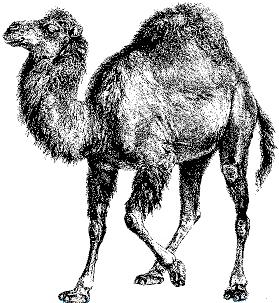
\includegraphics[width=0.15\textwidth]{c2_perl_logo_01.jpg}}
	  \item 优点:易于编程、快速成型、可移植性好、速度还可以、容易维护、……
	  \item 缺点:灵活、随意和“过度”的冗余语法、write-only、解释器耗费资源、……
	\end{itemize}
      \item 版本\textcolor{red}{(Perl5 vs. Perl6, Python2 vs. Python3)}
	\begin{itemize}
	  \item Perl5:1994年-至今,兼容性好、资源丰富
	  \item Perl6:2000年-至今,2015-12-25发布v1.0
	\end{itemize}
\parpic[fr]{
\includegraphics[width=0.15\textwidth]{c2_perl_logo_02.png}}
      \item 安装
%\parpic[fr]{
\includegraphics[width=0.15\textwidth]{c2_perl_logo_03.jpg}}
	\begin{itemize}
	  \item Unix/Linux:已经预装
	  \item Windows:Strawberry Perl,ActivePerl
	\end{itemize}
      \item 学习
	\begin{itemize}
	  \item 基本方法:文档、新闻组、邮件列表、FAQs、书籍、……
	  \item 书籍(生物信息学角度):\textit{Beginning Perl for Bioinformatics} $\Rightarrow$ \textit{Mastering Perl for Bioinformatics}
	  \item 书籍(编程语言角度):\textit{Learning Perl} $\Rightarrow$ \textit{Intermediate Perl} $\Rightarrow$ \textit{Mastering Perl} $\Rightarrow$ \textit{Programming Perl} $\Rightarrow$ \textit{Advanced Perl Programming}
	\end{itemize}
      \item \textcolor{red}{【重点】}基本语法\textcolor{red}{(演示实例操作)}
\vspace*{-10pt}
	\begin{multicols}{2}
\begin{verbatim}
#!/usr/bin/perl
use strict;
use warnings;
print "Hello World!\n";
\end{verbatim}
\begin{enumerate}
  \item 编写脚本,vim hello.pl
  \item 修改权限,chmod 755 hello.pl
  \item 运行脚本,perl hello.pl,./hello.pl
\end{enumerate}
\end{multicols}
\vspace*{-10pt}
      \item 其他:文本编辑器(Vim,插件:perl-support.vim);检查语法(perl -c script.pl);格式化代码(perltidy)
    \end{enumerate}
  \item \textcolor{red}{【重点、难点】}变量(15分钟)\textcolor{red}{(与队列、字典等进行类比,演示实例)}
    \begin{enumerate}
      \item 简介:Perl是一种无类型语言,不把变量分成整数、字符、浮点数等,只有一种能接受各种类型数据的“无类型”变量。
      \item 标量:scalar;只包含一个元素的变量;以 \verb|$|开头
	\begin{itemize}
	  \item 使用:\verb|$name="Paul";|,\verb|$age=29;|
	\end{itemize}
      \item 数组:array;含有任意数量元素的变量,以其存储顺序作为索引;以 \verb|@|开头
	\begin{itemize}
	  \item 初始化:\verb|@base=("A","C","G","T");|,\verb|@list=(1,2,3,4);|
	  \item 解引用:\verb|$base[0];|,\verb|$list[2];|
	  \item 操作函数:shift、unshift,pop、push
	\end{itemize}
      \item 散列:hash;把不同的变量按照逻辑关系组织起来,并以“键”作为索引;以 \verb|%|开头
	\begin{itemize}
	  \item 初始化:\verb|%person=(name => 'paul', age => '29');|
	  \item 提取键值:\verb|$person{"age"};|
	\end{itemize}
      \item 内置函数:\verb|$_|,\verb|$!|,\verb|@ARGV|,\verb|@_|,……
    \end{enumerate}

\otherTail
\newpage
\otherHeader

  \item 操作符(15分钟)
    \begin{enumerate}
      \item 数字操作符:\verb|+|,\verb|**|,\verb|%|,\verb|>|,\verb|!=|,\verb|<=>|,……
      \item 字符串操作符:\verb|.|,\verb|x|,\verb|gt|,\verb|ne|,\verb|cmp|,……
      \item 逻辑操作符:\verb|&&|,\verb=||=,\verb|!|,\verb|?=|,……
      \item 文件测试操作符:\verb|-r|,\verb|-e|,\verb|-s|,\verb|-f|,\verb|-T|,\verb|-M|,……
      \item 匹配操作符:\verb|=~|,\verb|!~|,\verb|~~|
    \end{enumerate}
  \item 基本函数(10分钟)
    \vspace*{-1em}
    \begin{multicols}{2}
    \begin{itemize}
      \item 打印输出:print
      \item 删除换行符:chomp
      \item 字符串操作:join,split
      \item 文件交互:open,close
      \item 目录操作:opendir,readdir,closedir
      \item 限定作用域:my
    \end{itemize}
  \end{multicols}
    \vspace*{-1em}
  \item 判断语句(10分钟)
    \begin{itemize}
\vspace*{-1em}
\begin{multicols}{2}
      \item if
\begin{verbatim}
if ($hour > 22) {
  print "should sleep...\n";
}

print "hello" if $guest >= 1;
\end{verbatim}
      \item unless
\begin{verbatim}
unless ($credit > 100) {
  print "You can not graduate!\n";
}
print "eat\n" unless $food==0;"
\end{verbatim}
\end{multicols}
\vspace*{-1em}
%\vspace{-1em}
\begin{multicols}{2}
      \item if-else
\begin{verbatim}
if ($name eq "Paul") {
  print "Hi Paul\n";
} elsif ($name eq "Joe") {
  print "Hi Joe\n";
} else {
  print "Who are you?";
}
\end{verbatim}
      \item given-when
\begin{verbatim}
use 5.010;

given ($foo) {
  say "a" when "a";
  when (/b/) {say "b";}
  default {say "not match";}
}
\end{verbatim}
\end{multicols}
\vspace*{-1em}
    \end{itemize}
  \item 循环语句(15分钟)
    \begin{itemize}
\vspace*{-1em}
\begin{multicols}{2}
      \item foreach
\begin{verbatim}
@group = 1..10;
foreach my $element (@group) {
  print "$element\n";
}
\end{verbatim}
      \item for
\begin{verbatim}
for ($i = 1; $i <= 10; $i++) {
  print "I can count to $i!\n";
}
\end{verbatim}
\end{multicols}
\vspace*{-1em}
\begin{multicols}{2}
      \item while
\begin{verbatim}
$i = 0;
while ($i < 10) {
  print "$i\n";
  $i++;
}
\end{verbatim}
      \item until
\begin{verbatim}
$i = 0;
until ($i == 10) {
  print "$i\n";
  $i++;
}
\end{verbatim}
\end{multicols}
\vspace*{-1em}
\begin{multicols}{2}
\item do-while\textcolor{red}{(比较while和do-while)}
\begin{verbatim}
$i = 0;
do {
  print "$i\n";
  $i = $i + 1;
} while ($i < 10);
\end{verbatim}
      \item do-until\textcolor{red}{(比较until和do-until)}
\begin{verbatim}
$i = 0;
do {
  print "$i\n";
  $i++;
} until ($i == 10);
\end{verbatim}
\end{multicols}
\vspace*{-1em}
    \end{itemize}

\otherTail
\newpage
\otherHeader

  \item 脚本检修(5分钟)
    \begin{enumerate}
      \item 好的习惯:\verb|use strict;|,\verb|use warnings;|
      \item 语法检查与格式化\textcolor{red}{(演示实例操作)}:\verb|perl -c script.pl|,\verb|perltidy script.pl|
      \item 脚本调试:\verb|perl -d script.pl|
    \end{enumerate}
  \item 总结与答疑(5分钟)
    \begin{enumerate}
      \item 知识点
	\begin{itemize}
	  \item Perl语言简介:基本知识,中心思想,语法结构,……
	  \item 变量:标量,数组,散列,内置变量
	  \item 操作符:数字,字符串,逻辑,文件测试,模式匹配
	  \item 基本函数:print,chomp,join,split,open,close,my
	  \item 判断语句:if,unless,given-when
	  \item 循环语句:foreach,for,while,until
	  \item 检修脚本:语法检查,代码格式化,脚本调试
	\end{itemize}
      \item 技能
	\begin{itemize}
	  \item 掌握Perl语言的基本语法
	  \item 使用Perl编写简单的应用脚本
	\end{itemize}
    \end{enumerate}
\end{enumerate}

\otherTail


\end{document}
